\documentclass[12pt, a4paper]{article}
\usepackage[utf8]{inputenc}
\usepackage[portuguese]{babel}
\usepackage{titlesec}
\usepackage{titling}
\usepackage{indentfirst}
\usepackage{graphicx}
\usepackage{wrapfig}
\usepackage{fancyhdr}
\usepackage{colortbl}
\usepackage{color}
\usepackage{framed}
\usepackage{enumitem}
\usepackage{amsmath}
\usepackage{listings}
\usepackage{lastpage}
\usepackage[hyphens]{url}
\usepackage{hyperref}
%\usepackage[brazilian,hyperpageref]{backref}
%\usepackage[num,overcite,abnt-emphasize=bf]{abntex2cite}
%%\usepackage[alf,abnt-emphasize=bf]{abntex2cite}
%%\citebrackets()
%\citebrackets[]

\graphicspath{{./images/}}
\definecolor{dkgreen}{rgb}{0,0.6,0}
\definecolor{gray}{rgb}{0.5,0.5,0.5}
\definecolor{mauve}{rgb}{0.58,0,0.82}

\lstset{frame=tb,
    language=C,
    aboveskip=3mm,
    belowskip=3mm,
    showstringspaces=false,
    columns=flexible,
    basicstyle={\small\ttfamily},
    numbers=none,
    numberstyle=\tiny\color{gray},
    keywordstyle=\color{blue},
    commentstyle=\color{dkgreen},
    stringstyle=\color{mauve},
    breaklines=true,
    breakatwhitespace=true,
    tabsize=4
}

\hypersetup{
    colorlinks=true,
    linkcolor=black,
    filecolor=magenta,      
    urlcolor=blue,
    citecolor=black,
}

%% Definindo o Autor e o título
\newcommand{\prof}{Rômulo César Silva}
\newcommand{\materia}{Algoritimos e Estruturas de dados}

\author{Victor Emanuel Almeida\and Milena Lucas Dos Santos\and Marco A. Guerra Pedroso}
\title{1$^{\underbar{o}}$ Trabalho de \materia}
\date{9 de março de 2021}

%% zera a pagina
\fancyfoot[C]{}
%% linhas no inicio e fim da página
\renewcommand{\headrulewidth}{0.7pt}
\renewcommand{\footrulewidth}{0.5pt}

\begin{document}
\begin{titlepage}
    \centering
    \thispagestyle{fancy}

    \begin{minipage}{0.4\textwidth}
        \begin{flushleft}
            
\includegraphics[scale=0.6]{logoUnioeste.jpeg}\\[1.0 cm]
        \end{flushleft}
    \end{minipage}
    \begin{minipage}{0.5\textwidth}
        \begin{flushright}\large
            \textsc{\LARGE\textbf{UNIOESTE}}\\
            \vspace{1cm}
            Universidade Estadual\\do Oeste do Paraná
        \end{flushright}
    \end{minipage}
    %\rule{\textwidth}{.5pt}\\[2.0 cm]
    \vspace*{4.5 cm}

    {\huge\bfseries\thetitle}\\
    \rule{\linewidth}{0.2 mm}\\[1.5 cm]

    \vspace{2cm}
    \begin{minipage}[t]{0.4\textwidth}
        \begin{flushleft}\large
            \emph{Professor:}\\
            \prof\\
        \end{flushleft}
    \end{minipage}
    \begin{minipage}[t]{0.5\textwidth}

        \begin{flushright}\large
            \emph{Grupo:}\\
            \theauthor
        \end{flushright}

    \end{minipage}\\[2 cm]

    \vfill\thedate
\end{titlepage}

\pagestyle{fancy}
%\fancyfoot[L]{Aluno(s):~\theauthor}
%\fancyfoot[R]{Prof:~\prof}
\fancyfoot[L]{}
\fancyfoot[R]{página~\thepage~de~\pageref{LastPage}}
\fancyhead[L]{}
\fancyhead[R]{}

\tableofcontents
\listoffigures
\newpage

\section{Estruturas de Dados}\label{Estruturas de Dados}
Todas as estruturas de dados estão definidas dentro da pasta ``./structures'', tendo como referência a raiz do projeto. As estruturas de dados implementadas são lista encadeada com cabeça e cauda no arquivo ``people\_list\_structure.h''e lista encadeada simples no arquivo ``registry\_structure.h''.
\subsection{Arquivo ``people\_list\_structure.h''}\label{Arquivo``peoplelist.h''}
\subsubsection{Estrutura ``Person''}\label{Estrutura ``Person''}
A estrutura ``Person'' armazena todos os dados para o cadastro dos habitantes, como também a prioridade desse habitante receber vacina e se já recebeu alguma dose da vacina.
\begin{lstlisting}
typedef struct {
    char *name;         // required
    int age;            // required
    char genre;         // required
    char *rg;           // required
    char *cpf;          // required
    char *phone;
    char *address;
    char *profession;
    short int priority; // required
    short int dose;
    struct vaccine *vaccine;
}Person;
\end{lstlisting}
\subsubsection{Estrutura ``Node''}\label{Estrutura ``Node''}
A estrutura ``Node'' define a lista encadeada, onde armazena a estrutura ``Person'' e o ``next'', ou seja, o ponteiro que aponta para a próxima pessoa.
\begin{lstlisting}
typedef struct node {
    Person data;
    struct node *next;
}Node;
\end{lstlisting}
\cleardoublepage
\subsubsection{Estrutura ``List''}\label{Estrutura ``List''}
A estrutura ``List'' define a cabeça e a cauda da lista encadeada.
\begin{lstlisting}
typedef struct {
    struct node *head;
    struct node *tail;
}List;
\end{lstlisting}
\subsection{Arquivo ``registry\_structure.h''}\label{Arquivo ``registry''}
\subsubsection{Estrutura ``Vaccine''}\label{Estrutura ``Vaccine''}
A estrutura ``Vaccine'' define o registro das vacinas e o ponteiro da próxima vacina.
\begin{lstlisting}
typedef struct vaccine {
    char *name;
    char *pharmaceutical;
    int inStock;
    struct vaccine *next;
}Vaccine;
\end{lstlisting}
\subsubsection{Estrutura ``Registry''}\label{Estrutura ``Registry''}
A estrutura ``Registry'' contém a lista para os habitantes, o registro da vacina e um \textit{int} validação do grupo prioritário.
\begin{lstlisting}
typedef struct {
    List *people;
    Vaccine *vaccine;
    int validGroup;
}Registry;
\end{lstlisting}
\cleardoublepage
\section{Uso do software}\label{Uso do software}
\subsection{Compilando o programa}\label{Compilando o proograma}
Todos os arquivos de implementação estão na pasta ``./sources'', sendo assim para realizar o processo de compilação em um sistema operacional que possui o compilador \textbf{GCC}, basta utilizar o comando ``\textbf{gcc main.c sources/*.c -o main}'' e após este comando executa-se o programa indicando o nome do arquivo de entrada, nesse caso chamado \textit{input} ``\textbf{main input}''.

Caso o sistema operacional não suporte a abreviação ``*.c'', segue abaixo a lista de todos os arquivos fontes contidos na pasta \textbf{sources}:
\begin{itemize}
    \item actions.c
    \item menu.c
    \item people\_list.c
    \item print\_stdio.c
    \item read\_file.c
    \item registry.c
    \item utils.c
    \item verify.c
\end{itemize}

\subsection{Execução do software}\label{Execução do software}
Para a execução do programa Sistema de Controle de Vacinas é apresentado uma tela inicial de interface mostrado na Figura \ref{telainicial}. O Menu Principal apresenta as funcionalidades do programa proposto, como cadastrar habitante, registrar vacinas, relatórios entre outros. Para percorrer por essas opções é necessário utilizar as teclas ``W'' e ``S'', pois ambas foram implementadas para percorrem pelas funcionalidades apresentadas. O Menu Principal é apresentado na Figura \ref{menu}. A opção para verificar os cadastros e registros de vacinas é a ``Emitir relatórios'', mostrado na Figura \ref{relatorio}. Desse modo, o programa é executado por meio do Menu Principal.

\cleardoublepage
\begin{figure}[h]
	\caption{Tela inicial do programa}
	
	\centering % para centralizarmos a figura
	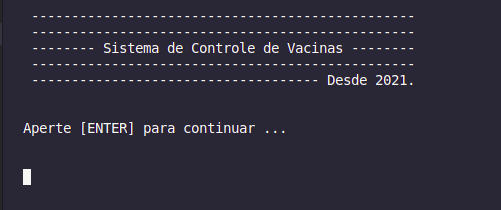
\includegraphics[width=10cm]{telaInicial.png} % leia abaixo
	\label{telainicial}
\end{figure}

\begin{figure}[h]
	\caption{Menu Principal}
	
	\centering % para centralizarmos a figura
	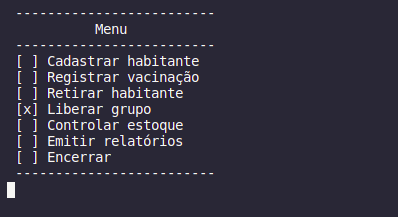
\includegraphics[width=10cm]{opcoes.png} % leia abaixo
	\label{menu}
\end{figure}

\begin{figure}[!h]
	\caption{Relatórios de cadastros e vacinas.}
	
	\centering % para centralizarmos a figura
	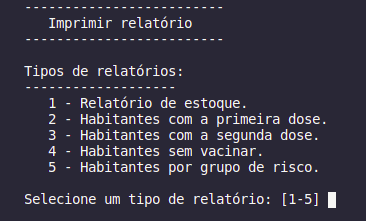
\includegraphics[width=10cm]{imprimirRelatorio.png} % leia abaixo
	\label{relatorio}
\end{figure}
\end{document}
